\chapter{Results} \label{chapResults}
\section{Photogrametry on Drone Forest Images}
A key first step in all the approaches we used is understanding the structure of the forest scene. The most flexible technique we used was structure from motion, since it only required uncalibrated images to obtain mesh representations of the environment. We found that the quality of the results depended heavily on the flight pattern that was used to collect the data. Automated over canopy lawnmower surveys performed the best and manual over canopy flights were slightly worse because of the lower density of observations and decreased consistency. Under canopy manual data collects had the worst results and often failed to properly identify the pose of many of the cameras. Results can be seen in Figure \ref{fig:results:sfm}.

\begin{figure}[H]
    \subfloat{\includegraphics[width=0.45\textwidth]{figs/results/geometric_understanding/stowe_anew_collect_000_zoomed_out.png}}
    \hfill
    \subfloat{\includegraphics[width=0.45\textwidth]{figs/results/geometric_understanding/stow_anew_collect_000_zoomed_in.png}}\\
        
    \subfloat{\includegraphics[width=0.45\textwidth]{figs/results/geometric_understanding/burn_zoomed_out.png}}
    \hfill
    \subfloat{\includegraphics[width=0.45\textwidth]{figs/results/geometric_understanding/burn_zoomed_in.png}}\\
    
    \subfloat{\includegraphics[width=0.45\textwidth]{figs/results/geometric_understanding/coimbra_zoomed_out.png}}
    \hfill
    \subfloat{\includegraphics[width=0.45\textwidth]{figs/results/geometric_understanding/coimbra_zoomed_in.png}}
    \caption{3D reconstructions using Agisoft Metashape on three different environments. The full map is shown to the left and a zoomed-in inset is shown to the right.}
    \label{fig:results:sfm}
\end{figure}

A practical consideration when working with these systems is the camera exposure. This is generally handled well by commodity systems, but may need to be hand-tuned on an experimental robotic system. If the exposure is too long, especially in the case of rapid drone movement, there can be motion blur which degrades the quality of reconstructions. Similarlly, both over and under-exposed images lead to fewer features to match between images and areas of minimial information in the final mesh.  

\subsection{SLAM in Forest Environments}

We validate our SLAM system by comparing it to the structure from motion result in Figure \ref{fig:results_mapping_slam}. This analysis was conducted solely by Dr. Francisco Yandun. 

\begin{figure*}[h!]
   \centering
   %----primera subfigura----
   \subfloat[]{
        \label{fig:metashape_cloud_baseline}         %% Etiqueta para la primera subfigura
        \includegraphics[width=0.465\textwidth]{figs/results/geometric_understanding/metashape_cloud_v3.png}}
   %\hspace{0.1\linewidth}
   \subfloat[]{
        \label{fig:slam_orig_1}         %% Etiqueta para la segunda subfigura
        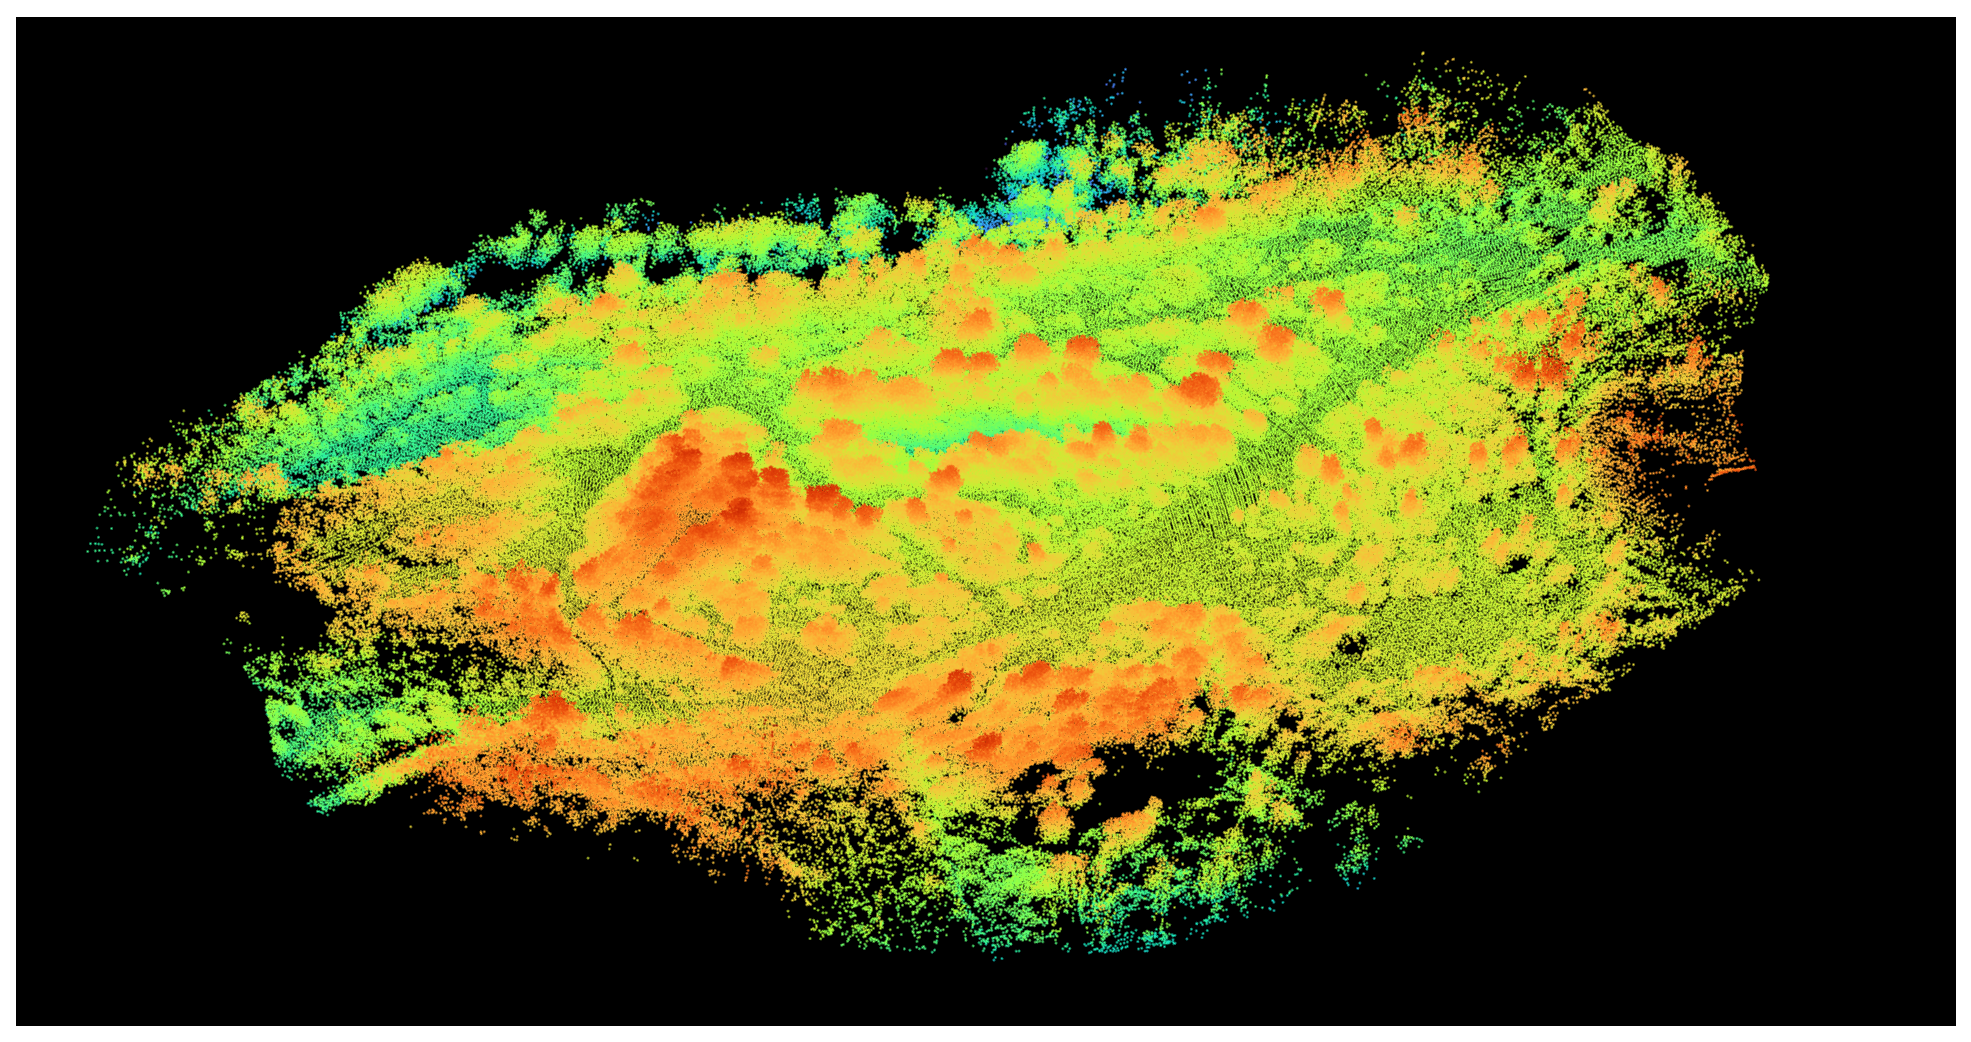
\includegraphics[width=0.5\textwidth]{figs/results/geometric_understanding/slam_ptCloud.eps}}\\%\\[20pt]   
   \subfloat[]{
        \label{fig:slam_hausdorff}         %% Etiqueta para la segunda subfigura
        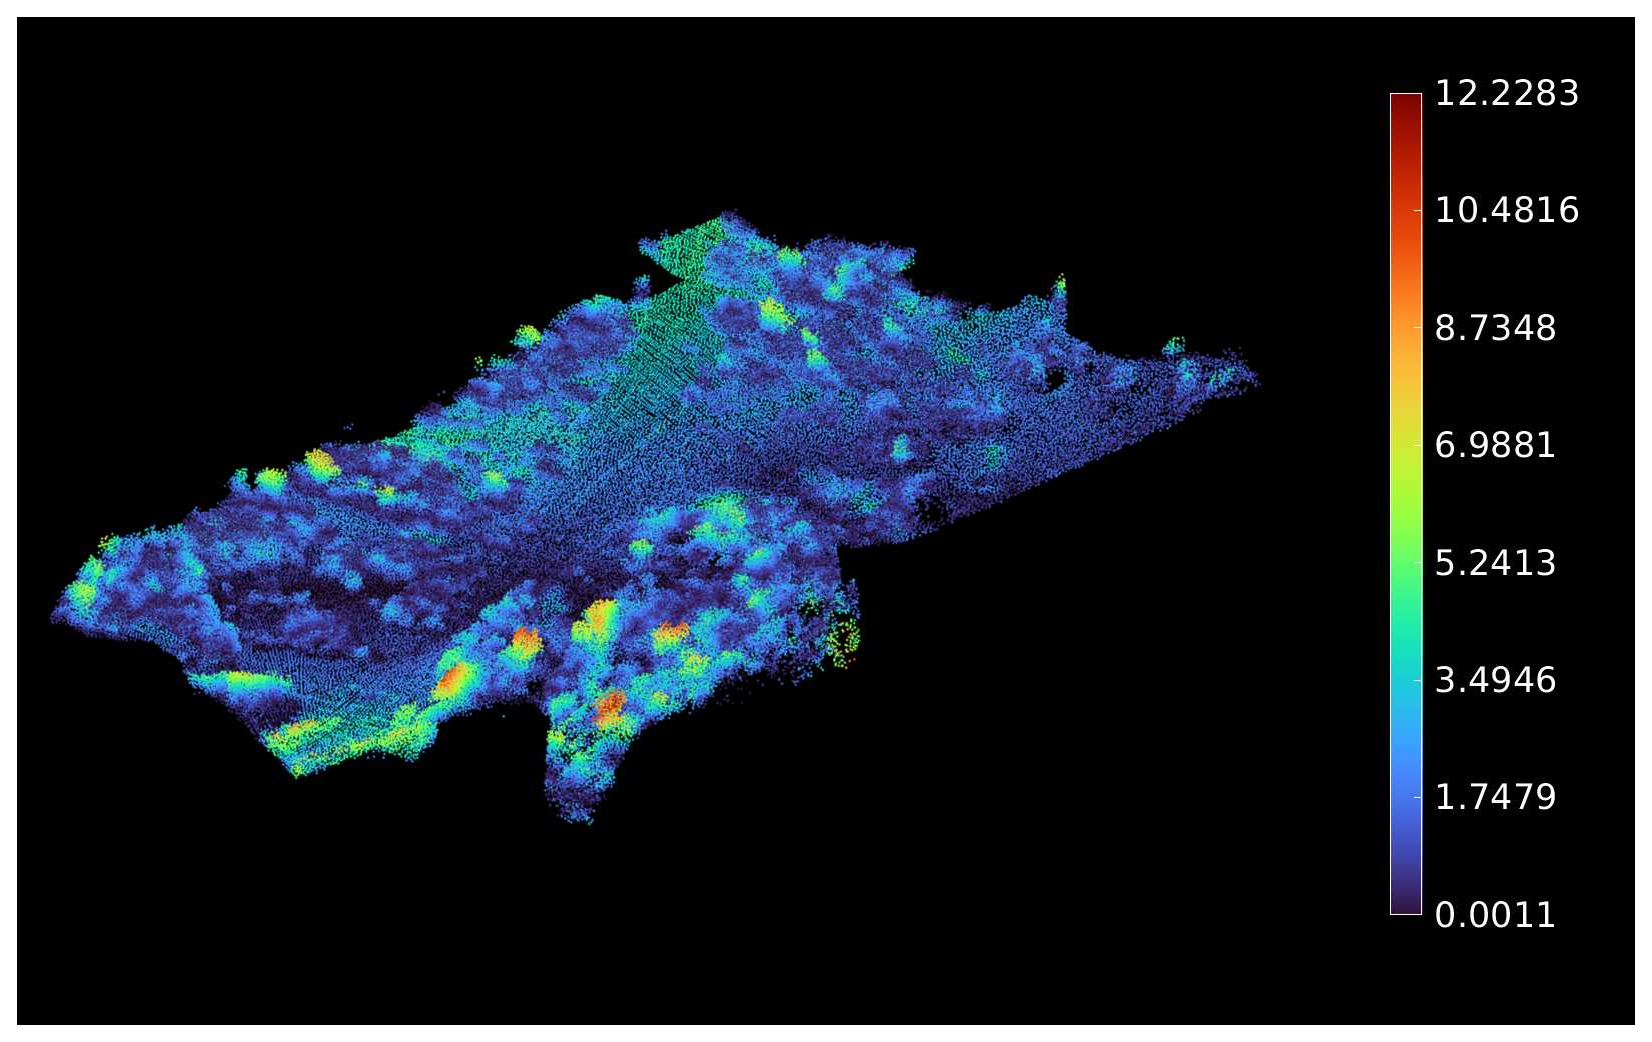
\includegraphics[width=0.5\textwidth]{figs/results/geometric_understanding/housedorff_distance.eps}}%\\[20pt]            
   \caption{Point cloud maps of the A) photogrammetry baseline, B) SLAM outcome. The two maps were compared using the Hausdorff distance, whose result is visualized as C) the SLAM map colored according to this metric. Note that the baseline and the SLAM clouds colormaps correspond to RGB and height values, respectively. Figure courtesy of Dr. Francisco Yandun.}
   \label{fig:results_mapping_slam}                %% Etiqueta para la figura entera
\end{figure*}

\begin{itemize}
    \item Talk more about the way SLAM was run
    \item Talk more about the comparison
\end{itemize}


\section{Semantic mapping}
An unfortunate challenge of semantic mapping is that it's nearly impossible to collect a groundtruth representation without survey-grade equiptment and extensive annotation resources. Therefore, we perform most of our quantitative evaluation purely on the images, and show only qualitative results from the final semantic map. 

\subsection{Image Segmentation}



\subsubsection{Sete Fonte experiment}

\begin{figure}
    \centering
    \includegraphics[width=0.7\columnwidth]{figs/results/semantic_segmentation/confusion_matrix.pdf} 
    \caption{Confusion matrix for the \textit{Setes Fontes} test datasets normalized per class with the true fraction of each class reported on the y axis labels.
    %Fuel is predicted fairly well, though it is fairly often confused for canopy, which is understandable given the visual similarity and the large fraction of canopy pixels.
    }
    \label{fig:semantics_confusion}
\end{figure}
\begin{figure}
   % First row
   \centering
    \includegraphics[width=\linewidth]{figs/results/semantic_segmentation/SeteFontes/qualatative_001400.png}  
    \includegraphics[width=\linewidth]{figs/results/semantic_segmentation/SeteFontes/qualatative_001600.png}  
    \caption{Predictions on the \textit{Oporto} dataset. Black is background, red is fuel, brown is trunks, and green is canopy.
    %Note that low trees are often predicted as fuel.
    } 
    \label{fig:qualitative_semantics_semfire}
\end{figure}

We conducted experiments to determine how many real training images were needed, with and without synthetic pretraining, as seen in Figure \ref{fig:results:semantic-size-pretraining}. We used mean Intersection over Union (mIoU) to evaluate the quality of the predictions on the test set. It is interesting to note the relatively high performance of a model that used only 7 real images. Also, the model trained solely on synthetic data fails to generalize to real data, even after properly accounting for differences in mean and variance of both datasets. We found that combined real and synthetic data performs worse than training the same model only using real data. This suggests that the synthetic data comes from a completely different distribution than the real one, making its contribution detrimental. In the future, we plan to keep researching the causes of this interesting outcome.

\begin{figure}
    \centering
    \includegraphics[width=0.7\textwidth]{figs/results/semantic_segmentation/synthetic_experiments_mious.pdf}
    \caption{Test mIoU for very few training images on the \textit{Setes Fontes} dataset.
    Error bars represent minimum and maximum result across the five folds of \textit{Setes Fontes}.}
    \label{fig:results:semantic-size-pretraining}
\end{figure}

As the model trained in 121 images ($80\%$ of the \textit{Setes Fontes} dataset) showed the best performance and was used for deployment in the \textit{Oporto} dataset, which was never seen during training.
%Qualitative examples of both can be seen in Figure \ref{fig:qualitative_semantics_semfire} and
The confusion matrix on the \textit{Setes Fontes} test set can be found in Figure \ref{fig:semantics_confusion} and qualitative results are in Figure \ref{fig:qualitative_semantics_semfire}. As we are mainly interested in the fuel instances, we aggregated the background, trunks, and canopies in a single non-fuel class. In that case we obtained an IoU of 78.2\% and 95.3\% for \texttt{Fuel} and \texttt{Not Fuel}, respectively, which yields a mIoU of 86.7\%. This shows that our system performs well at its primary task of identifying fuel.



\subsubsection{Gascola experiment}
We evaluated our model by training it on data from one flight and testing it on another. Because of the images we chose, these two datasets had different class distributions as shown in Figure \ref{fig:results:semantic_class_fracs}, though they had the same three main classes. Each of these three classes corresponded to a different aggregate class, so it was important to effectively tell them apart. 


\begin{figure*}[h!]
   \centering
   %----primera subfigura----
   \subfloat[]{
        \label{fig:train_class_frac}         %% Etiqueta para la primera subfigura
        \includegraphics[width=0.5\textwidth]{figs/results/semantic_segmentation/class_fraction_train.png}}
   %\hspace{0.1\linewidth}
   \subfloat[]{
        \label{fig:test_class_frac}         %% Etiqueta para la segunda subfigura
        \includegraphics[width=0.5\textwidth]{figs/results/semantic_segmentation/class_fraction_test.png}}%\\[20pt]            
   \caption{This shows the fraction of pixels per class for A) the train set and B) the test set. Note that the three dominant classes Canopy, Bare Earth, and Dry Grass are common across both collections but the comparative frequencies are somewhat different. These correspond to our aggregate Canopy, Background, and Fuel classes respectively. The fractions of other classes are fairly small, and some from the training set are entirely absent in the test set.}
   \label{fig:results:semantic_class_fracs}                %% Etiqueta para la figura entera
\end{figure*}

The quality of predictions is shown in Table \ref{tab:results:semantic_eval}. The the performance is fairly good on the most common classes, but, as expected drops on the rarer classes. As seen by the qualitative examples in Figure \ref{fig:results:semantic_gascola_qualitative}, there are instances where the predictions on the granular classes are incorrect, but the aggregate class is correct.

\begin{table}[ht!]
    \centering
\begin{tabular}{ccccc}
% \hline
\toprule
\textbf{Class} & \textbf{IoU} & \textbf{Precision} & \textbf{Recall} \\ \midrule
% \hline
Canopy & 70.05 & 84.77 & 80.13 \\
Dry Grass & 79.7 & 93.75 & 84.17 \\
Bare Earth & 78.53 & 88.12 & 87.83 \\
Green Shrubs & 3.27 & 21.72 & 3.71 \\
Green Grass & 0.0 & 0.0 & 0.0 \\
Dry Shrubs & 0.0 & 0.0 & 0.0 \\
Live Trunks & 0.05 & 0.05 & 84.09 \\
\bottomrule
% \hline
\end{tabular}
\caption{Evaluation results of the SegNext network with the Anderson Fuel Model as a base for semantic segmentation in a forestry environment.}
\label{tab:results:semantic_eval}
\end{table}


\begin{figure*}[h!]
   \centering
   \includegraphics[width=0.5\textwidth]{figs/results/semantic_segmentation/Gascola/safeforest_all_classes_flat.png}
   \includegraphics[width=0.25\textwidth]{figs/results/semantic_segmentation/Gascola/safeforest_classmap_compressed_flat.png}
   
\includegraphics[width=0.80\textwidth]{figs/results/semantic_segmentation/Gascola/000000_rgb_img.png}
   \vspace{0pt}
   
\includegraphics[width=0.80\textwidth]{figs/results/semantic_segmentation/Gascola/000005_rgb_img.png}
   \vspace{0pt}
   
\includegraphics[width=0.80\textwidth]{figs/results/semantic_segmentation/Gascola/000010_rgb_img.png}
   \vspace{0pt}
   
\includegraphics[width=0.80\textwidth]{figs/results/semantic_segmentation/Gascola/000015_rgb_img.png}
   \vspace{0pt}
   \caption{
   Qualitative semantic mapping results from the test set. The results are shown both for the predicted classes and the aggregated ones, with colors visualized in the top rows.
   White regions in the ground truth represent areas that were ambiguous to the human annotator. Overall the predictions match the ground truth well and boundaries are well-defined. Note that many regions of confusions, such as canopy-to-trunk and green shrub to canopy, fall within the same coarse classes for our mapping purposes.
   }
   \label{fig:results:semantic_gascola_qualitative}                %% Etiqueta para la figura entera
\end{figure*}

\subsection{Projecting Segmentation into 3D}
The final goal of semantic mapping is to develop a model of the environment and what class different regions are. To evaluate the feasibility of this, we conduct two experiments using multi-sensor data.

The first experiment uses data that we collected under the canopy using a payload inclination of 30 degrees from horizontal. The drone was manually piloted to survey the perimeter of a clearing. We the best model described in the previous Gascola section to generate predictions on the images and localization from the vision-LiDAR SLAM system from \cite{RussellUnmannedMitigation}. The results are shown in Figure \ref{fig:semantic_SLAM_result}. This shows that the system was able to determine that there was significant fuel at ground level and correctly identify the tree trunks in the environment. The later is important because they could be used as a localization aid in a similar way to SLOAM \cite{Chen2020SLOAM:Inventory}. One issue that we observed was that multiple scans were not perfectly registered to each other. This is in contrast to the final pointcloud derived from SLAM, where fine details are captured preciseslly. Our hypothesis is that because the SLAM system uses a pose-graph \cite{Dellaert2017FactorPerception} formulation, information from loop closures can be used to update the historical pose to make it more accurate. However, the semantic mapping system only uses the most recent SLAM pose estimate, which is likely to be less accurate than the final optimzed version.

\begin{figure}
    \centering
    \includegraphics[width=0.8\textwidth]{figs/results/semantic_mapping/semantic_cloud_first_approach.png}
    \caption{Semantic mapping results on the Oporto test site. Fuel is red, trunks are green, canopy is purple, and background is black. White points are unlabeled.}
    \label{fig:results:semantic_mapping_original}
\end{figure}

In our second experiment, we sought to evaluate the performance more objectively. This is challenging because accurate field-reference data is challenging to acquire. Instead, we choose to label an ortho-mosoaic derived from a 3D model by hand. We used QGis\footnote{\url{https://qgis.org/en/site/}}, an open-source software for interacting with geospatial data. We labeled three coarse classes, fuel, canopy and background, which included bare-earth and other non-flammable material. This manual process took approximately eight hours to complete and is visualized on the left side of Figure \ref{fig:results:semantic_map_UFO}.

We used the SLAM output from LIO-SAM to provide the estimated pose. In this case, we used a the UFOMap version of semantic mapping developed primarily by Duda Andrada. There results of this are shown in Figure \ref{fig:results:semantic_map_UFO}. The overall structure of the scene matches well and small local features are correctly identified. One major source of error is seen in the miss-registration of data from adjacent drone flights. This is seen in the vertical offsets that are especially visible on the left side of the map. This may be due to latency in the processing or also because of using the un-refined pose as described previously. The quality of this result suggests that with additional work to properly register the scans, this system could be a powerful tool for vegitation mappng. 

\begin{figure}
    \centering
    \includegraphics[width=0.45\textwidth]{figs/results/semantic_mapping/labeled_orthomoasaic.png}
    \includegraphics[width=0.45\textwidth]{figs/results/semantic_mapping/segnext_gc5_ufomap.png}
    \caption{Manually-labeled result on the left, result from UFO-Map on the right provided by M. Duda Andrada, using the semantic segementation model described previously. }
    \label{fig:results:semantic_map_UFO}
\end{figure}


\section{Tree Detection}
The goal of this study is to understand the quality of tree predictions in satellite versus drone data. We also wanted to explore how much improvement a small set of annotations could yeild. Finally, we wanted to see how best to predict trees in a large expanse of satellite data using only a small number of labeled trees and a drone datasets collected around them.

The first step in this processes was processing the drone images into an orthomosaic, as described in the Photogrametry section. The orthomosiac was roughly geospatially regestered from the GPS readings where each image was taken. However, we noticed a translational error of several meters when the orthomosaic was overlaid on the NAIP data. Fixed translatinoal offsets are a common error with consumer GPS, though scale and rotation are often much more accurate. We fix this issue manually using an overlay in QGis to estimate the translational offset, and then updating the metadata using `gdalwarp`  


In the first experiment, we simply


Our work shows that the tree detection results are substantially better on drone data compared to NAIP as shown in Figure \ref{fig:results:tree_det}. However, the quality of NAIP detections can be improved substantially by finetuning the model on only a small amount of data.

\begin{itemize}
    \item TODO expand this
    \item TODO the most important figure to add is probably a table of metrics for the different approaches.
    \item TODO Talk about how many trees get detected as multiple smaller ones. This could be a histogram of sqrt areas. 
\end{itemize}

\begin{figure}[h]
    \subfloat{\includegraphics[width=0.45\textwidth]{figs/results/tree_detections/stowe_anew_base.png}}
    \hfill
    \subfloat{\includegraphics[width=0.45\textwidth]{figs/results/tree_detections/stowe_anew_retrained.png}}
    \vfill
    \subfloat{\includegraphics[width=0.45\textwidth]{figs/results/tree_detections/NAIP_base.png}}
    \hfill
    \subfloat{\includegraphics[width=0.45\textwidth]{figs/results/tree_detections/NAIP_retrained.png}}
    \caption{Tree detections on an orthomosiac (top) and NAIP data (bottom). The left column shows the DeepForest predictions without any retraining, while the right column shows the results after retraining on a small amount of local annotations.}
    \label{fig:results:tree_det}
\end{figure}


\section{Informative path planning}

\begin{figure}[h]
    \subfloat{\includegraphics[width=0.45\textwidth]{figs/results/ipp/unpaired_qual_1 (1).png}}
    \hfill
    \subfloat{\includegraphics[width=0.45\textwidth]{figs/results/ipp/unpaired_qual_2 (1).png}}
    \caption{Visualizations of the proposed planning method on two different data images.}
    \label{fig:res_unpairqual}
\end{figure}


\begin{figure}[h]
    \subfloat{\includegraphics[width=0.45\textwidth]{figs/results/ipp/paired_qual_GBS-IPP (1).png}}
    \hfill
    \subfloat{\includegraphics[width=0.45\textwidth]{figs/results/ipp/paired_qual_pizza (1).png}}
    \caption{A comparison of the proposed method with a baseline}
    \label{fig:res_pairedqual}
\end{figure}

\begin{figure}[h]
    \subfloat{\includegraphics[width=0.3\textwidth]{figs/results/ipp/error (2).png}}
    \hfill
    \subfloat{\includegraphics[width=0.3\textwidth]{figs/results/ipp/balanced_error (2).png}}
    \hfill
    \subfloat{\includegraphics[width=0.3\textwidth]{figs/results/ipp/timing_result (1).png}}
    \caption{Quantitative statistics for IPP. TODO replace with updated ones.}
    \label{fig:res_ipp_quant}
\end{figure}

\subsection{Evaluation}
\begin{itemize}
    \item TODO explain the qualitative differences in paths, e.g. it stays in more varied areas longer
    \item TODO explain
\end{itemize}

The experiments demonstrate a small but significant improvement in both error metrics from the proposed, as can be seen in Figure~\ref{fig:quant}. It should be noted that the variance of both approaches were high, which highlights the need for further experiments.

As seen in Figure~\ref{fig:pairqual}, when run on the same data, the proposed approach is able to come up with a plan that yields a more representative sample of the environment, compared to the baseline. Further examples of the proposed planning method run on image data can be seen in Figure~\ref{fig:unpairqual}. 

An interesting finding is that the performance of both approaches did not improve dramatically over the sampling iterations. This can likely be attributed to the simple prediction model we used which saturated quickly. The performance of the proposed planner was especially stable. This suggests that it was able to very quickly saturate the prediction model by choosing a representative set of samples in the first round.The performance would probably increase more over time if we used a more complex prediction system, instead of nearest neighbor. 

The timing results, seen in the leftmost part of Figure~\ref{fig:quant}, show that the algorithm can plan a mission in approximately 100 seconds using a laptop with a RTX3700 GPU. This shows that this approach is extremely feasible for deployment under operational constraints. An interesting finding is that the timing does not increase significantly over iterations. This is interesting because during the uncertainty estimation portion of the approach we use an increasingly-large Gaussian Process. We expected that the order $n^3$ time of this step would dominate the system runtime, but this was not the case. We will further profile the system timing in future work.


